\chapter{Attributes}
\label{ch:attributes}

\section{Attributes of antifragile}
\label{sec:attributesantifragile}

\begin{figure}[h!]
	\centering
	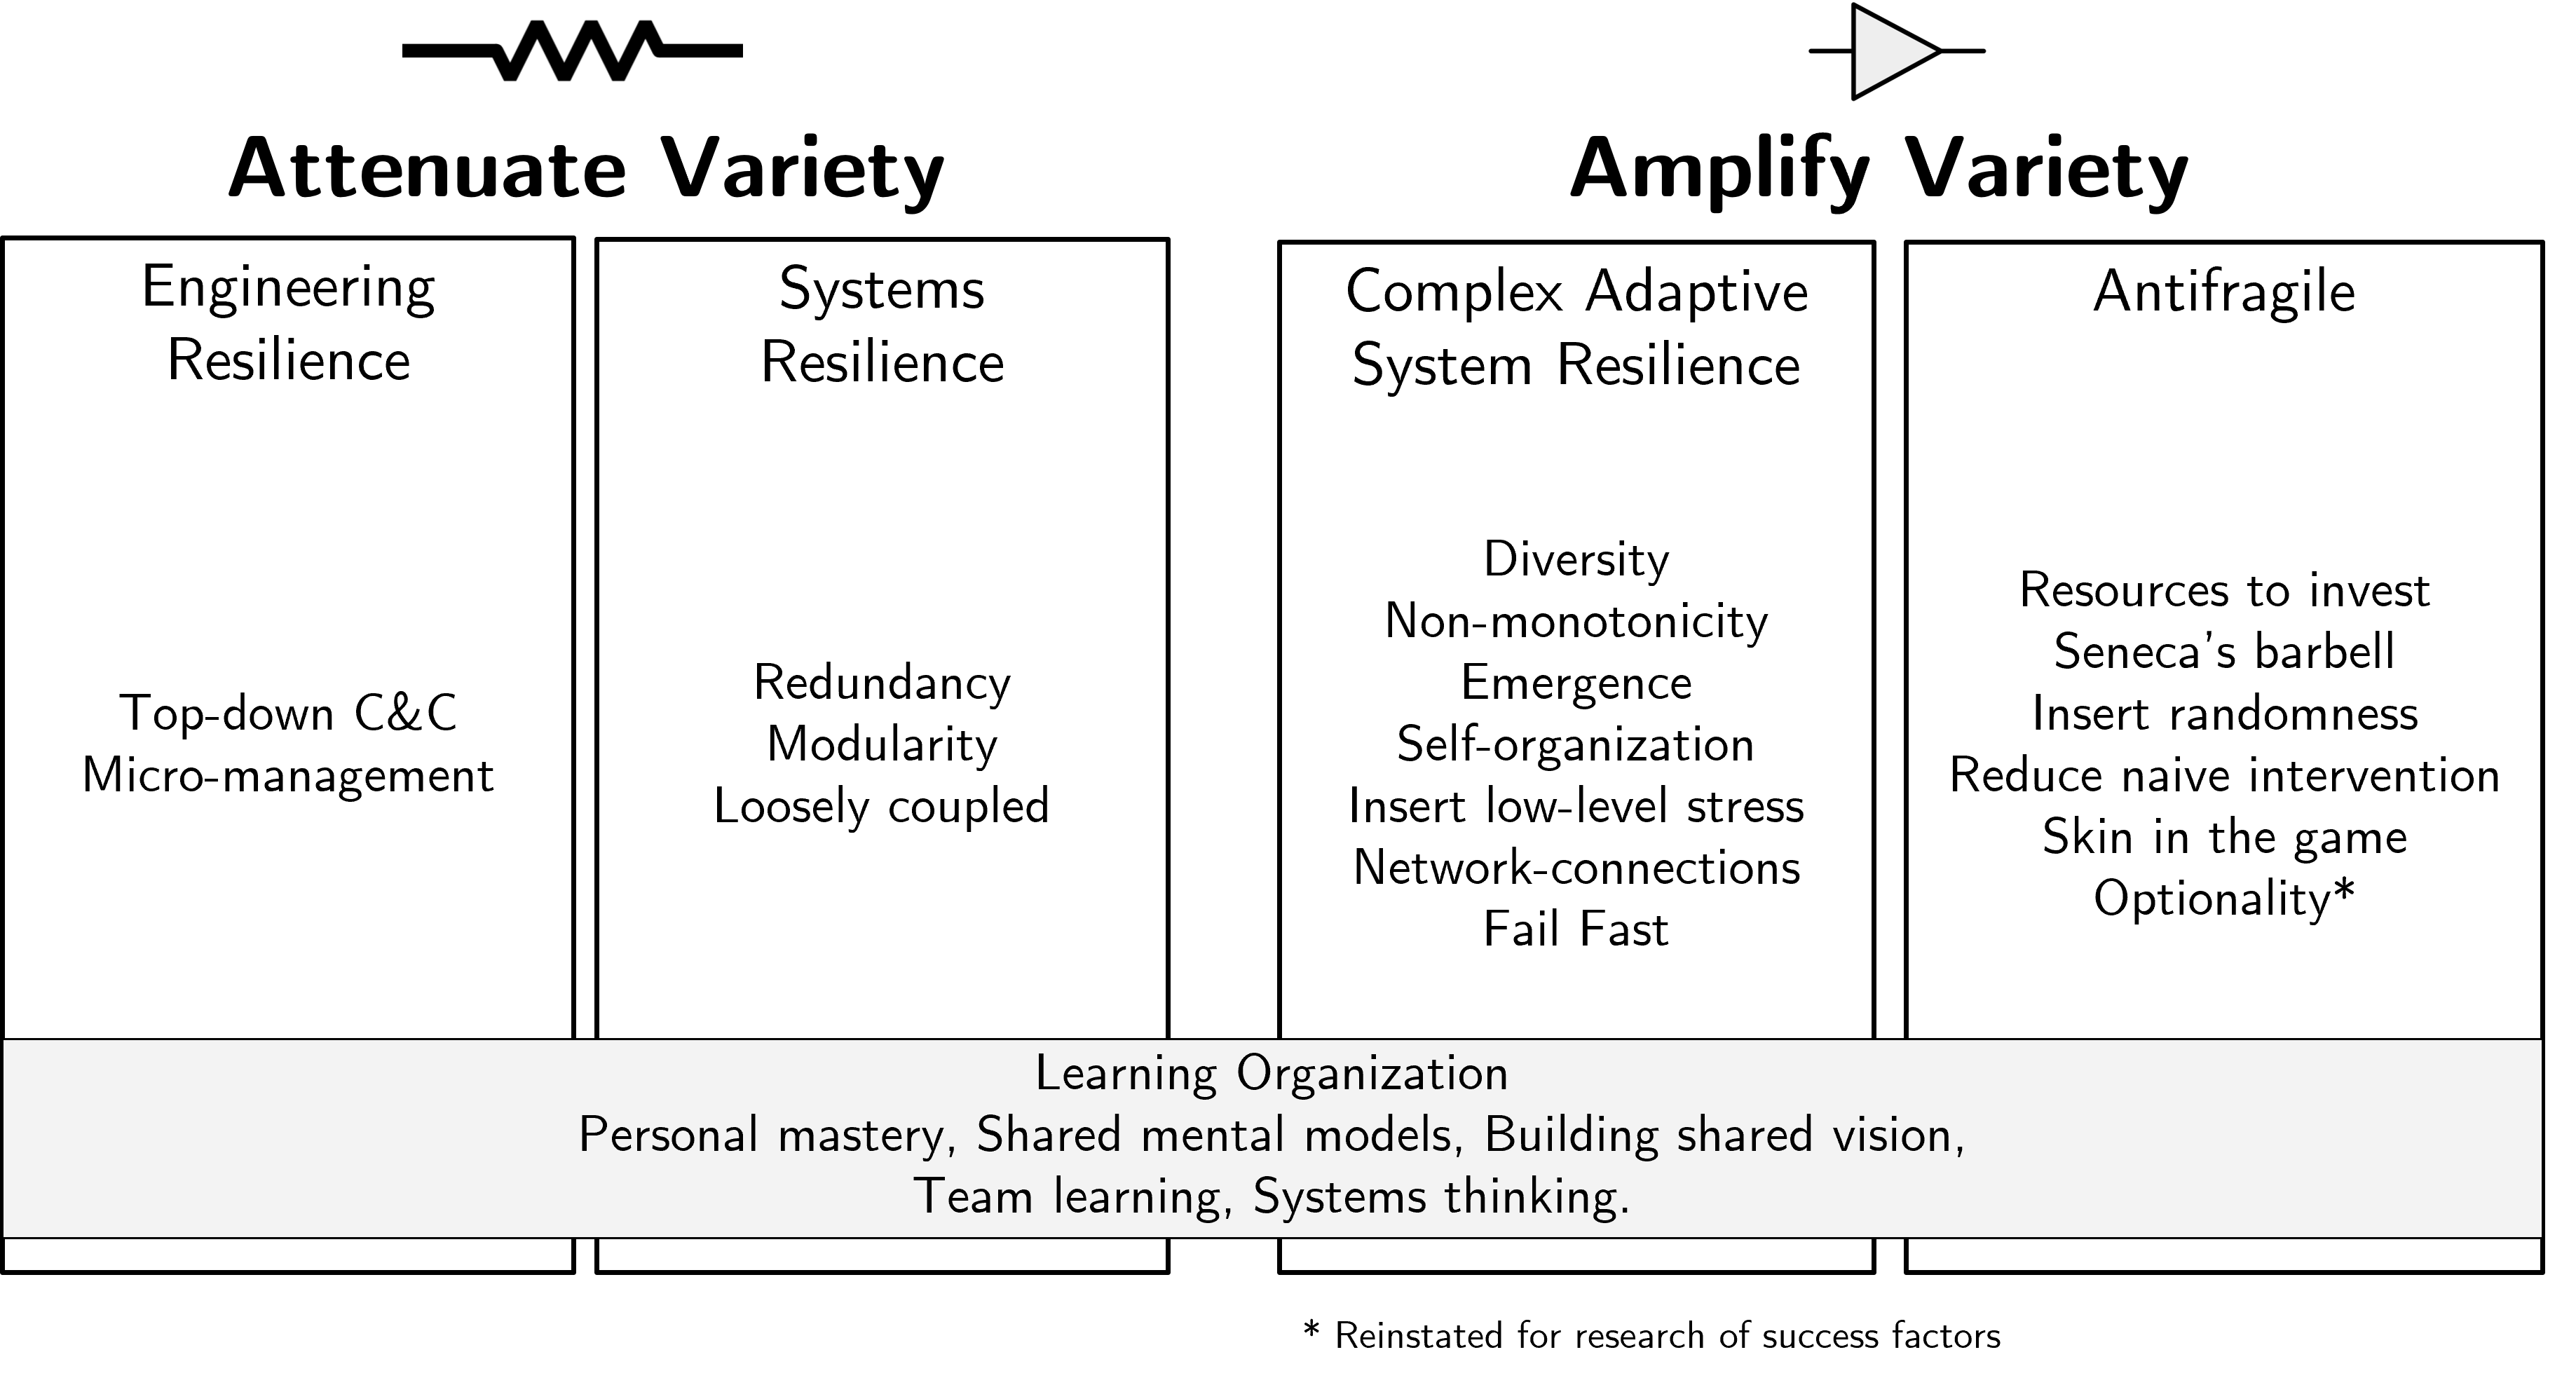
\includegraphics[width=0.8\linewidth]{images/eaalbwincludingoptionality}
	\caption[Extended Antifragile Attribute List \parencite{Botjes2021} with Optionality]{Extended Antifragile Attribute List \parencite{Botjes2021} with Optionality}
	\label{fig:eaalbwincludingoptionality-attributes}
\end{figure}

\subsection{\Gls{attenuatevariety} attributes}
\begin{table}[H]
	\begin{center}
			\begin{tabular}{@{}ll@{}}
			\toprule
				\textbf{Attribute} & \textbf{Sources} \\%
				\midrule%
				Top Down C\&C & \parencite{Botjes2020} \\%
				Micro-Management & \parencite{Botjes2020} \\%
				Redundancy & \parencite{Botjes2020} \\%
				Modularity & \parencite{Botjes2020} \\%
				Loosely coupled & \parencite{Botjes2020} \\%
			\bottomrule%
			\end{tabular}
			\caption[Attenuating attributes of \gls{antifragile}]{Attenuating attributes of \gls{antifragile}}
			\label{tab:attenuatingattributes}
\end{center}
\end{table}				

\subsection{\Gls{amplifyvariety} attributes}
\begin{table}[H]
	\begin{center}
		\begin{tabular}{@{}ll@{}}
			\toprule
			\textbf{Attribute} & \textbf{Sources} \\%
			\midrule%
			\Gls{diversity} & \parencite{Botjes2020} \\%
			\Gls{optionality} & \parencites{Taleb2012}{Gorgeon2015} \\%
			\Gls{nonmonotonicity} & \parencite{Botjes2020} \\%
			\Gls{emergence} & \parencite{Botjes2020} \\%
			\Gls{selforganisation} & \parencite{Botjes2020} \\%
			\Gls{insertlowlevelstress} & \parencite{Botjes2020} \\%
			\Gls{networkconnections} & \parencite{Botjes2020} \\%
			\Gls{failfast} & \parencite{Botjes2020} \\%
			\Gls{resourcestoinvest} & \parencites{Taleb2012}{Botjes2020} \\%
			\Gls{senecabarbell} &  \parencites{Taleb2012}{Botjes2020} \\%
			\Gls{insertrandomness} & \parencites{Taleb2012}{Botjes2020} \\%		
			\Gls{reducenaiveintervention} & \parencites{Taleb2012}{Botjes2020} \\%
			\Gls{skininthegame} & \parencites{Taleb2012}{Botjes2020} \\%
			\bottomrule%
		\end{tabular}
		\caption[Amplifying attributes of \gls{antifragile}]{Amplifying attributes of \gls{antifragile}}
		\label{tab:amplifyingattributes}
	\end{center}
\end{table}			

\subsection{\Gls{attenuatevariety} and \gls{amplifyvariety} attributes}

\begin{table}[H]
	\begin{center}
		\begin{tabular}{@{}ll@{}}
			\toprule
			\textbf{Attribute} & \textbf{Sources} \\%
			\midrule%
			\Gls{personalmastery} & \parencite{Botjes2020} \\%
			\Gls{sharedmentalmodels} & \parencite{Botjes2020} \\%
			\Gls{buildingsharedvision} & \parencite{Botjes2020} \\%
			\Gls{teamlearning} & \parencite{Botjes2020} \\%
			\Gls{systemsthinking} & \parencite{Botjes2020} \\%
			\bottomrule%
		\end{tabular}
		\caption[Attenuating and amplifying attributes of \gls{antifragile}]{Attenuating and amplifying attributes of \gls{antifragile}}
		\label{tab:attenuatingandamplifyingattributes}
	\end{center}
\end{table}	

\section{Attributes of Enterprise Architecture}
\label{sec:attributesonea}

\subsection{Enterprise IT Architecting attributes}
\label{sub:enterpriseitarchitecting}
\begin{table}[H]%
	\begin{center}%
		\begin{tabular}{@{}ll@{}}%
			\toprule%
			\textbf{Attribute} & \textbf{Sources} \\%
			\midrule%
			 & \parencite{Lapalme2012} \\%
			\bottomrule%
		\end{tabular}%
		\caption[Attributes of Enterprise Ecological Adaptation]{Attributes of Enterprise Ecological Adaptation}%
		\label{tab:attributesofenterpriseitarchitecting}%
	\end{center}%
\end{table}%


\subsection{Enterprise Integrating attributes}
\label{sub:attributesofenterpriseintegrating}
\begin{table}[H]%
	\begin{center}%
		\begin{tabular}{@{}ll@{}}%
			\toprule%
			\textbf{Attribute} & \textbf{Sources} \\%
			\midrule%
			 & \parencite{Lapalme2012} \\%
			\bottomrule%
		\end{tabular}%
		\caption[Attributes of Enterprise Integrating]{Attributes of Enterprise Integrating}%
		\label{tab:attributesofenterpriseintegrating}%
	\end{center}%
\end{table}%

\subsection{Enterprise Ecological Adaptation attributes}
\label{sub:enterpriseecologicaladaptation}

\begin{table}[H]
	\begin{center}
		\begin{tabular}{@{}ll@{}}
				\toprule
				\textbf{Attribute} & \textbf{Sources} \\%
				\midrule%
				\Gls{systeminenvironment} & \parencite{Lapalme2012} \\%
				\Gls{holisticsystemicstance} & \parencite{Lapalme2012} \\%
				\Gls{intraorganisationalcoherency} & \parencite{Lapalme2012} \\%
				\Gls{organisationallearning} & \parencite{Lapalme2012} \\%
				\Gls{environmentallearning} & \parencite{Lapalme2012} \\%
				\Gls{systeminenvironmentcoevolutionlearning} & \parencite{Lapalme2012} \\%
				\bottomrule%
			\end{tabular}
		\caption[Attributes of Enterprise Ecological Adaptation]{Attributes of Enterprise Ecological Adaptation}
		\label{tab:attributesofeea}
	\end{center}
\end{table}


